% !TeX spellcheck = it_IT
%Carattere dimensione 12
\documentclass[12pt]{report}

\usepackage[italian]{babel} % conversione in italiano
\usepackage{libertine}
\usepackage{graphicx}
\usepackage{amsmath}
\usepackage{pgfplots}
\usepackage{amssymb}
\usepackage{bm} % fornisce il comando \bm per il testo in grassetto
\usepackage[utf8]{inputenc}
\usepackage{float} % aggiunge l'opzione H alle "floating figures"
\usepackage{alphalph} % permette di generare lettere dato un indice numerico
\usepackage{minted} % highlighting del codice
\usepackage{xcolor} % importa colori predefiniti


% \usepackage[strict]{changepage}
% \usepackage{floatflt}
% \usepackage{blindtext}
% \usepackage{enumitem}
% \usepackage{amsthm}
% \usepackage{subfig}
% \usepackage{listings}
% \usepackage{listingsutf8}
% \usepackage{framed}
% \usepackage{minibox}
% \usepackage{wrapfig}
% \usepackage{longtable}

\usepackage{standalone}
\usepackage{tikz}
\usepackage{caption, setspace}
\usepackage{hyperref}
\usepackage{import}
\usepackage{booktabs}
\usepackage{array} 
\usepackage{subcaption}
\usepackage{algorithmicx}
\usepackage[noend]{algpseudocode}
\usepackage[chapter]{algorithm}

\hypersetup{ % enable hyperlinks
    colorlinks,
    citecolor=black,
    filecolor=black,
    linkcolor=black,
    urlcolor=black
  }
% \usepackage{csquotes}


\pgfplotsset{width=11cm,compat=1.9}
\usepgfplotslibrary{external}
\usetikzlibrary{external}
\usetikzlibrary{positioning}
\usetikzlibrary{arrows}
\usetikzlibrary{calc}
\tikzexternalize%


\usepackage[top=3cm, bottom=3cm, left=3cm, right=3cm]{geometry}
\pagestyle{plain}
\linespread{1.5}
\captionsetup{margin=10pt,font={small},labelfont=bf} % caption styling


\usepackage[backend=biber, sorting=none]{biblatex}
\addbibresource{references.bib}

% \definecolor{funcolor}{HTML}{ef8a62} %TODO: externalize styles
\definecolor{funcolor}{HTML}{427ef5} %TODO: externalize styles

\newcommand{\includetikz}[2]{%
  \centering%
  \scalebox{#1}{\input{#2}}%
}

\newenvironment{dedication}
{\vspace*{50ex}\begin{quotation}\begin{center}\begin{em}}
      {\par\end{em}\end{center}\end{quotation}}

\subimport{./layers/}{init}

\begin{document}
% \selectcolormodel{cmyk}
\begin{titlepage}
  \begin{figure}[t]
    %\centering
\includegraphics[width=0.9\textwidth]{marchio-unipi.eps}
    \centering\includegraphics[width=0.9\textwidth]{./img/logo.eps}

    \vspace{1cm}

    \centering\includegraphics[width=0.4\textwidth]{./img/cherubino.eps}
  \end{figure}

  \begin{center}
    \textbf{ Dipartimento di Informatica\\ Corso di Laurea Triennale in Informatica\\}
    \vspace{15mm}
    {\LARGE{\bf Localizzazione Indoor Basata su Beacon Bluetooth a Bassa Potenza
        Attraverso Tecniche di Deep Learning}}\\
  \end{center}

  \vspace{20mm}

  \begin{minipage}[t]{0.47\textwidth}
    {\large{\bf Relatore:\\ Prof.\ GianLuigi Ferrari 
        % \\ Prof. Alessio Micheli
      }}
  \end{minipage}\hfill
  \begin{minipage}[t]{0.47\textwidth}\raggedleft
    {\large{\bf Presentata da: \\ Marco Pampaloni}}
  \end{minipage}

  \vfill


  \centering{\large{\bf Anno Accademico 2019/2020 }}

\end{titlepage}

\begin{abstract}
  \documentclass{standalone} 
\begin{document}
I sistemi di localizzazione indoor, ovvero i sistemi che permettono la
localizzazione di dispositivi all’interno di un ambiente chiuso, dove non è
possibile sfruttare la copertura del sistema GPS, sono stati oggetto di
notevole interesse. Questo elaborato illustra una soluzione tecnologica al
problema della localizzazione indoor basata sull’uso di strumenti di machine
learning. La soluzione proposta sfrutta una rete neurale convoluzionale (CNN)
profonda. I dati di input del modello costituiscono una serie temporale di
segnali broadcast \emph{Bluetooth Low Energy} (BLE) emessi da un insieme di
Beacon disposti all’interno dell’edificio oggetto della Localizzazione Indoor,
mentre l’output è una coppia di coordinate relative alla posizione all’interno
dell’edificio stesso. La soluzione inoltre utilizza alcune tecniche di
\emph{data augmentation} per generare un dataset di grandi dimensioni sulla
base dei campionamenti dei segnali effettuati in loco.

A seguito dell’addestramento, il modello utilizzato ha mostrato un errore medio
assoluto (MAE) sul dataset di test pari a \emph{30cm}, esibendo una buona
affidabilità anche rispetto a variazioni significative dei segnali dovute al
rumore ambientale. Per ridurre ulteriormente l’errore medio  è stato costruito
un insieme di modelli, ognuno addestrato con diversi iperparametri. Questa
tecnica ha permesso di ridurre l’errore medio fino a circa \emph{26cm}.

Il modello prodotto risulta eseguibile in tempo reale su dispositivi mobile con
ridotte capacità computazionali, rendendolo particolarmente adatto alla
cosiddetta navigazione ``blue-dot'' all’interno di contesti Indoor. Tuttavia la
variazione dell’output del modello ha originato una navigazione poco fluida.
Per arginare questo problema è stato applicato un filtro di Kalman al modello e
viene sfruttato il sensore inerziale dello smartphone per produrre un’euristica
utile a individuare i movimenti dell’utente.
\end{document}

\end{abstract}

% Dedica
\clearpage
\begin{dedication}
  \thispagestyle{empty}
  A Snoopy
\end{dedication}
\clearpage
\pagenumbering{arabic}

\tableofcontents

\chapter{Introduzione}
\documentclass{standalone}
\begin{document}
%Problema
\section{Localizzazione Indoor}
Il problema della Localizzazione Indoor consiste nell'individuazione di un
utente all'interno di uno spazio chiuso e in riferimento a un sistema di
coordinate predefinito. Tale sistema di coordinate, relativo ad un determinato
edificio, può essere poi espresso in termini georeferenziali conoscendo la
precisa dislocazione geografica del locale in questione. \\
La localizzazione indoor apre le porte a diverse possibilità nel campo
dell'esperienza utente all'interno di edifici pubblici, nel settore
della gestione dei flussi di persone, della sicurezza e della contingentazione.
Attraverso l'impiego di tale tecnologia è possibile coadiuvare la navigazione
degli utenti all'interno di edifici complessi e migliorare l'esperienza
individuale di persone affette da disabilità. Per ottenere questi risultati è
però richiesto un certo grado di precisione, di affidabilità, di efficienza e
di sicurezza nella gestione della privacy dei dati di localizzazione degli
utenti. Inoltre la tecnologia scelta per risolvere il problema, per essere
fruibile, deve avere come ulteriore requisito il basso impatto economico.

\section{Soluzioni Tecnologiche}
%Letteratura
Nel corso degli anni sono state implementati diversi sistemi di
localizzazione indoor, che possiamo dividere in due macrocategorie: soluzioni
ad-hoc e soluzioni che sfruttano tecnologie esistenti. Nel primo caso si
fornisce all'utente l'attrezzatura necessaria ad essere localizzato, mentre nel
secondo si utilizza un dispositivo mobile di proprietà dell'utilizzatore.
Spesso tale dispositivo è uno smartphone. \\ I sistemi che implementano
tecnologie sviluppate ad-hoc, sono spesso più efficienti, più precisi e
flessibili. Tuttavia il loro impiego rimane limitato dall'alto costo di
progettazione, installazione e di gestione. È poi richiesto che ad ogni utente
che intende essere localizzato sia assegnato un dispositivo che si interfacci
col sistema impiegato. \\
Per l'impiego su larga scala, un sistema di localizzazione indoor deve essere
facilmente utilizzabile dalle masse e non deve richiedere particolari requisiti
tecnologici.  \\

{\LARGE TODO: Inserire riferimenti bibliografici che mettano in comparazione le
  varie tecnologie utilizzate, ad-hoc e non, e in particolare mostrino i
  risultati dei sistemi che sfruttano il Bluetooth.}

\section{Bluetooth Low Energy}
La tecnologia \emph{Bluetooth} è talmente pervasiva che
ogni smartphone in circolazione ne implementa il protocollo, mostrandosi
particolarmente adeguata alla risoluzione del problema in esame. Nello
specifico, \emph{Bluetooth Low Energy} (BLE) è un protocollo che riduce
notevolmente il consumo energetico dei dispositivi che ne sfruttano le
capacità. \\
La soluzione riportata in questo documento prevede l'utilizzo di una serie di
beacon BLE programmabili, ciascuno installato in un punto significativo
dell'edificio e configurato per emettere un segnale broadcast con una frequenza
di circa 50Hz. La potenza dei segnali viene quindi utilizzata per produrre,
attraverso l'utilizzo di una rete neurale artificiale, una coppia di coordinate
rappresentative della posizione dell'utente all'interno dell'edificio. Ciò
viene reso possibile da una fase preliminare in cui viene mappata la superficie
del locale raccogliendo i segnali ricevuti dai beacon in vari punti. Per ogni
punto della superficie mappato si registra una serie temporale di segnali, dei
quali si considera solo il valore \emph{RSSI}, ovvero la potenza del segnale
nel punto in cui questo viene ricevuto. \\
Il modello utilizzato è di fatto completamente agnostico rispetto
all'ubicazione dei beacon installati, fin quando questa sia unica e non mutata
nel tempo. \\
L'utilizzo di tale sistema assicura il completo anonimato dell'utente, il quale
non necessita di condividere la propria posizione, essendo quest'ultima
calcolata direttamente sul suo smartphone in funzione dei segnali che riceve.

% Contenuto
Questa tesi si pone l'obiettivo di descrivere nello specifico la rete neurale
progettata per risolvere il problema, le tecniche utilizzate per alzare il
grado di precisione del modello e le principali differenze rispetto a modelli
già esistenti.


\end{document}


\chapter{Deep Learning}
\documentclass{standalone}

\begin{document}
In questo capitolo saranno introdotti i concetti fondamentali alla base delle
moderne tecniche di Deep Learning e le strutture matematiche necessarie alla
loro comprensione. \\

\section{Machine Learning}
Il \emph{Machine Learning}, o apprendimento automatico, è un insieme di
tecniche e algoritmi che consentono a dei programmi di ``imparare'' a svolgere
un determinato compito sulla base di esperienze pregresse, senza bisogno da
parte del programmatore di specificare come eseguire tale mansione. 
\subsection{Regressione Lineare}
Un esempio classico di algoritmo di machine learning è quello della regressione
lineare. Scopo dell'algoritmo è quello di predire l'output di una determinata
funzione.  Si consideri quindi un vettore $ \bm x \in \mathbb{R}^n $, e
un valore scalare $\hat{y} = \bm \theta^\intercal \bm x$. il
vettore $\bm \theta$ introduce i parametri del modello, mentre
$\hat{y}$ ne rappresenta l'output, che è una funzione lineare di $\bm
x$. Siano quindi $ \bm x_1, \bm x_2, \dotsc, \bm x_m $ dei vettori in
$\mathbb{R}^n$ e  $ y_1, y_2, \dotsc, y_m $ i corrispettivi valori della
funzione $f(\bm x_i)$ che stiamo cercando di approssimare.

Perchè la funzione $\hat{y}(\bm x)$ approssimi $f(\bm x)$ è necessario che i
parametri $\bm \theta$ del modello si adattino in modo da minimizzare la differenza
tra l'output prodotto dal modello e la cosiddetta \emph{ground truth}: $y =
f(\bm x)$. A questo scopo si definisce una metrica di errore propria del
processo di apprendimento: l'errore quadratico medio (MSE dall'inglese) 
$$MSE = \frac{1}{m} \sum_{i=1}^m{(\hat{y} - y_i)^2}$$

Per minimizzare l'errore sul nostro dataset di test è sufficiente porre a zero
la derivata, rispetto a $\bm \theta$, della nostra funzione di costo. Nel caso
della regressione lineare è possibile risolvere l'equazione risultante
ottenendo un sistema di equazioni che prende il nome di 
\emph{normal equations}.
Esistono tuttavia metodi numerici iterativi che si basano sulle informazioni
fornite dal gradiente della funzione di costo che permettono di aggiornare i
parametri del modello cercando di ridurne l'errore, anche nel caso di modelli
non lineari. L'algoritmo su cui si basano molti dei moderni metodi di
apprendimento del Deep Learning è il \emph{gradient descent} o metodo del
gradiente.

Il metodo del gradiente aggiorna i parametri $\bm \theta$ del modello secondo
la seguente regola: 
$$ \bm \theta' = \bm \theta - \eta \nabla_{\bm \theta} J(\bm \theta) $$
dove $J(\bm \theta)$ rappresenta la funzione di costo associata al modello,
mentre $\eta$ è un coefficiente chiamato \emph{learning rate}.
%Intuizione gradient descent
Un'interpretazione dell'algoritmo è data dalle informazioni sulla monotonia
ottenute dal gradiente della funzione di costo: per $\eta$ abbastanzza piccolo
risulta $J(\bm \theta') \leq J(\bm \theta)$ poichè il gradiente negativo di $J$
determina la direzione di massima decrescita della funzione\cite{goodfellow}.
Ne consegue che applicando ricorsivamente la regola di aggiornamento del metodo
del gradiente, la nostra funzione $\hat{y}$ tenderà ad avvicinarsi alla
funzione originale $y$, minimizzando la funzione di costo.
Possiamo intepretare il coefficiente $\eta$ come la velocità con cui seguire la
pendenza della funzione di errore.

%Gradient descent con MSE e modello lineare
Nel caso di un modello di regressione lineare che usa l'MSE come funzione di
costo, risulta: 
\begin{align*}
  &\forall j \in {1, \dotsc, n}: \\
  %
  \frac{\partial}{\partial\theta_j} MSE
  &= 
  \frac{\partial}{\partial\theta_j} \frac{1}{m} \sum_{i=1}^m{(\hat{y}_i -
    y_i)^2} \\ 
  %
  &= \frac{\partial}{\partial\theta_j} \frac{1}{m}
  \sum_{i=1}^m{(\bm \theta^\intercal \bm x_i - y_i)^2} \\
  %
  &= \frac{1}{m}
  \sum_{i=1}^m{\frac{\partial}{\partial\theta_j}(\bm \theta^\intercal \bm x_i -
    y_i)^2} \\
  %
  &= \frac{2}{m}
  \sum_{i=1}^m{(\bm \theta^\intercal \bm x_i - y_i)x_i^{(j)}}
\end{align*}
%
Ovvero abbiamo che la regola di aggiornamento è:
$$ \theta'_j = \theta_j - \eta \frac{\partial}{\partial\theta_j} J(\bm \theta)
             = \theta_j - \eta (\frac{2}{m} 
             \sum_{i=1}^m{(\bm \theta^\intercal \bm x_i - y_i)x_i^{(j)}}),
             \quad \forall j \in \{1, \dotsc, n\}
$$


% \section{Multi Layer Perceptron}


\end{document}



\chapter{Architettura Software}\label{cap:architecture}
\begin{document}
\newcommand{\yhatone}{\bm\hat{\bm y}_1}
\newcommand{\yhattwo}{\bm\hat{\bm y}_2}
\newcommand{\yold}{\bm y_{\mathit{old}}}
In questo capitolo è descritta nel dettaglio l'architettura software sviluppata
per il progetto di locallizazione indoor, inclusa la rete neurale, le librerie
utilizzate, gli ambienti di sviluppo e gli strumenti che hanno coadiuvato il
testing e la sperimentazione del prototipo realizzato.
\section{TensorFlow}
%%%%%%%%%%%%%%%%%%%%%%%%%%%%%%%%%%%%%%%%%%%%%%%%%%%%%%%%%%%%%%%%%%%%%%%%%%%%%%%
\section{Keras}
%%%%%%%%%%%%%%%%%%%%%%%%%%%%%%%%%%%%%%%%%%%%%%%%%%%%%%%%%%%%%%%%%%%%%%%%%%%%%%%
\section{Google Colab}
%%%%%%%%%%%%%%%%%%%%%%%%%%%%%%%%%%%%%%%%%%%%%%%%%%%%%%%%%%%%%%%%%%%%%%%%%%%%%%%
\section{Weights \& Biases}
%%%%%%%%%%%%%%%%%%%%%%%%%%%%%%%%%%%%%%%%%%%%%%%%%%%%%%%%%%%%%%%%%%%%%%%%%%%%%%%
\section{Architettura della Rete Neurale}
\begin{figure}[!htp]
  % \makebox[\textwidth][c]{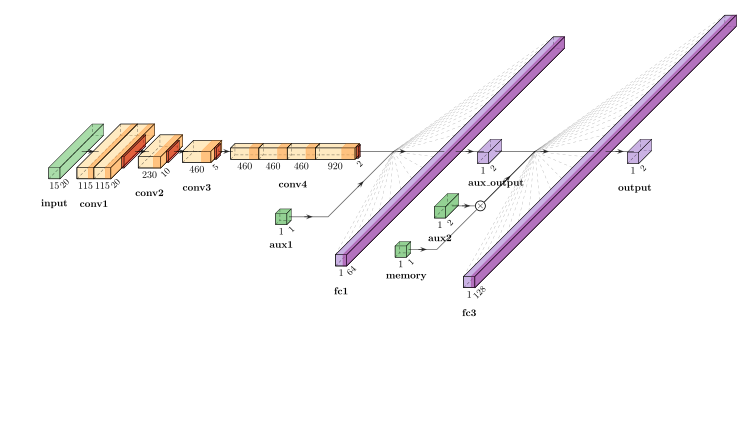
\includegraphics[width=1.0\textwidth]{./img/architettura.pdf}}%
  \makebox[\textwidth][c]{%
    \includetikz{0.75}{./img/architettura}%
  }%
  % 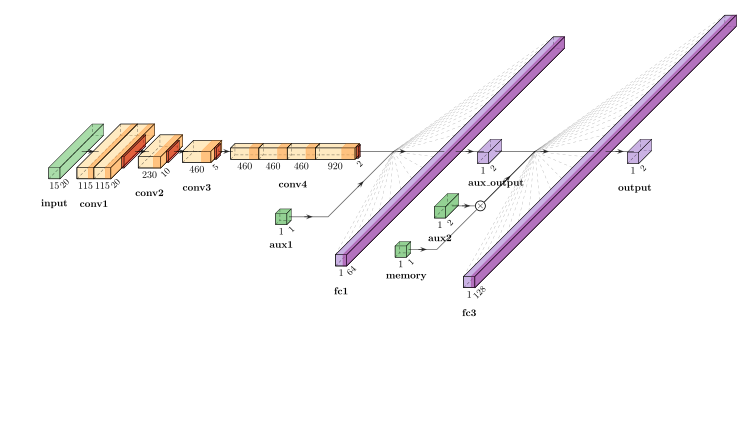
\includegraphics[width=1.3\textwidth]{./img/architettura.pdf}
  % \includetikz{0.8}{./img/architettura.tex}
  \caption{Architettura della rete neurale}%
  \label{fig:crynet}%
\end{figure}
La rete neurale sviluppata per il problema di localizzazione indoor è
illustrata schematicamente in Figura~\ref{fig:crynet}. Essa consiste in una
serie di blocchi convoluzionali seguiti da alcuni livelli di neuroni
completamente connessi. Il modello sfrutta, oltre ai segnali RSSI emessi dai
beacon, anche due input ausiliari che non sono processati dalla sezione
convoluzionale della rete.
\subsection{Input del Modello}
L'input principale del modello è composto da una serie temporale di valori RSSI
relativi ai segnali emessi da 15 beacon disposti lungo il perimetro
dell'edificio nel quale si sono svolte le sperimentazioni del prototipo. La
dimensione temporale dell'input può essere arbitrariamente lunga, poichè una
sua variazione determina solamente una differente dimensione dell'asse
temporale dell'output della CNN\@. La sezione convoluzionale della rete si
conclude infatti con un livello di pooling globale che consiste
nell'estrazione, per ogni feature map prodotta, della media aritmetica dei
valori di input lungo la dimensione del tempo. Come si vede in
Figura~\ref{fig:crynet}, infatti, la dimensione dell'output di tale livello è
sempre costante e risulta essere $920\times1$.

A completare l'input del modello sono il valore emesso dal sensore magnetico
dello smartphone e l'ultima posizione nota dell'utente all'interno
dell'edificio, indicati rispettivamente con \(\alpha\) e \( \yold \). Il
valore della bussola è utile per determinare l'orientamento della persona nello
spazio, rendendo la rete neurale capace di considerare le variazioni dei
segnali BLE dovuti all'assorbimento da parte del corpo dell'utilizzatore dello
smartphone. Il secondo input ausiliario è invece utilizzato per correggere
eventuali scostamenti rilevanti dell'output della CNN rispetto alla posizione
precedente dell'utente. Ci si aspetterebbe infatti che tale posizione non
variasse di molto in un lasso di tempo breve.

L'ultima posizione nota dell'utente viene pesata da un coefficiente, anche esso
input del modello, che in Figura~\ref{fig:crynet} è indicato con la lettera
greca \(\mu\). Tale valore, cui possiamo riferirci con il termine
\emph{coefficiente di memoria residua}, è compreso tra zero e uno, e determina
il peso che si vuole dare all'ipotesi di continuità della posizione dell'utente
nel tempo.  \(\mu = 0\) indica l'assenza di tale assunzione, con la conseguente
massima riduzione della correzione dell'output della CNN da parte dei livelli
successivi, mentre \(\mu = 1 \) associa il massimo peso su tale ipotesi. Il
coefficiente di memoria residua è esso stesso input del livello successivo
della rete, il quale riceve anche i valori dell'output ausiliario e di 
\(\mu \cdot \yold\).

Il valore della bussola è input del primo livello completamente connesso,
insieme all'output della CNN\@.
\subsection{Blocco Convoluzionale}
La prima parte del modello è una semplice rete neurale convoluzionale
unidimensionale. Sebbene sia composto da due dimensioni, quella temporale e
quella dei beacon, quest'ultima può essere interpretata come l'insieme dei
canali della prima, come nel caso dei canali \emph{r}, \emph{g}, \emph{b} di
un'immagine a colori. Ciò permette di applicare l'operazione di convoluzione
soltanto lungo l'asse temporale.
La CNN proposta è composta da otto blocchi convoluzionali consecutivi così
strutturati:
\begin{itemize}
    \item Operazione di convoluzione sull'output del livello precedente
    \item Funzione di attivazione ReLU sull'output della convoluzione
    \item Livello di batch normalization
\end{itemize}
Un esempio di blocco convoluzionale è illustrato in Figura~\ref{fig:cnnblock},
mentre in Figura~\ref{fig:crynet} sono mostrati anche i livelli di pooling,
rappresentati da una superficie rossa apposta accanto i blocchi convoluzionali.
\begin{figure}
  \makebox[\textwidth][c]{%
    \includetikz{0.75}{./img/cnnblock}%
  }%
  \caption{Singolo blocco convoluzionale: la parte chiara indica l'operazione
    di convoluzione, mentre l'ombreggiatura sulla destra illustra la funzione
    di attivazione ReLU. \(K\) è il numero di filtri utilizzati e di
    conseguenza equivale al numero di feature map prodotte, mentre \(N\) è la
    lunghezza della serie temporale. Il processo di Batch normalization è
    omesso dalla schematizzazione.}%
  \label{fig:cnnblock}%
\end{figure}

L'output del secondo, terzo e quarto blocco convoluzionale sono sottoposti
ciascuno all'applicazione di un particolare metodo di dropout chiamato
\emph{dropout gaussiano}. Esso consiste nell'applicare del rumore
moltiplicativo, con distribuzione gaussiana di media unitaria, all'output del
blocco convoluzionale. Lo scopo è quello di simulare una corruzione casuale dei
dati di addestramento del modello, con l'obiettivo di regolarizzare
quest'ultimo. Applicare il rumore all'output dei livelli intermedi della rete,
piuttosto che al dataset iniziale, consente di manipolare più profondamente la
rappresentazione dei dati imparata dal modello, rendendolo conseguentemente più
robusto rispetto alle variazioni dei segnali di
input\cite{noise-hidden-layers}. Gli effetti dell'utilizzo del dropout
gaussiano sono illustrati in Tabella~\ref{tab:nogaussdrop}.
\begin{table}[tbp]
  \centering
  \begin{tabular}{lcccc}
    \toprule
    Modello & Loss & MAE & RMSE & MaxAE \\
    \midrule
    Baseline      & 0.7796 & 0.3070 & 0.6716 & 3.001 \\
    Senza G.Dropuout & 0.8911 & 0.3171 & 0.7138 & 3.256 \\
    \bottomrule
  \end{tabular}
  \caption{Modello \emph{baseline} messo a confronto con una versione dello
    stesso che non utilizza il dropout gaussiano. Le metriche fanno riferimento
      al dataset di \emph{test}.}%
  \label{tab:nogaussdrop}%
\end{table}


L'output dell'ultimo blocco convoluzionale è infine seguito da un livello di
pooling globale e dall'applicazione del dropout.
\subsection{Uso della Bussola e Output Ausiliario}
L'utilizzo dei valori forniti dal sensore magnetico dello smartphone sono
giustificati dal voler mitigare il cosiddetto effetto del \emph{body
  shadowing}.  Tale fenomeno si verifica quando un segnale wireless si propaga
in un ambiente e collide contro un corpo umano. Tale collisione provoca un
decadimento del segnale, il quale arriva disturbato al punto di ricezione. Ciò
influisce sulla precisione dei sistemi di localizzazione indoor basati sui
valori RSSI dei segnali wireless in modo considerevole, poichè è sufficiente che
l'utente volti le spalle a un sottoinsieme dei beacon attivi per introdurre
rumore all'interno del sistema. Utilizzando il valore emesso dalla bussola
dello smartphone, è possibile rendere il modello consapevole dell'orientamento
dell'utente e attenuare il rumore introdotto dal \emph{body shadowing}. I
risultati ottenuti dall'utilizzo di questo input sono illustrati in
Tabella~\ref{tab:nocompass}, la quale mette in relazione il modello finale con
uno che non considera l'input della bussola.
\begin{table}[htp]
  \centering
  \begin{tabular}{lcccc}
    \toprule
    Modello & Loss & MAE & RMSE & MaxAE \\
    \midrule
    Baseline      & 0.7796 & 0.307 & 0.6716 & 3.001 \\
    Senza Bussola & 1.619 & 0.447 & 0.9784 & 4.5 \\
    \bottomrule
  \end{tabular}
  \caption{Varie metriche a confronto per i due modelli in esame:
    \emph{Baseline} è il modello finale, mentre il secondo differisce dal primo
    soltanto dall'uso dei valori della bussola, che vengono semplicemente
    scartati. Le metriche si riferiscono al dataset di \emph{test}, ovvero al
    processo di valutazione successivo alla fase di addestramento.}%
  \label{tab:nocompass}%
\end{table}


L'input corrispondente al sensore magnetico è un valore scalare \(\alpha \in
  \mathbb{R}, \) con \(0 \leq \alpha \leq 360\), in cui il valore \(0\) indica
il nord. Tale dato è fornito, come mostrato in Figura~\ref{fig:crynet}, al
primo livello completamente connesso della rete, insieme all'output della
CNN\@.  Questo livello produce un vettore di 64 elementi, il quale diventa
input del secondo livello completamente connesso del modello. L'output di
quest'ultimo livello, indicato in figura come \(\yhatone\), è una coppia
di coordinate reali che indica la posizione dell'utente all'interno
dell'edificio.  Tale previsione è soltanto parziale, in quanto non tiene conto
dell'ultima posizione nota dell'utente, ma risulta utile per guidare
l'addestramento del modello verso una soluzione meno dipendente da tale input.
A questo scopo \(\yhatone\) è interpretrato dal modello come output
ausiliario.

A ogni output ausiliario è associata una funzione di costo, il cui valore va
poi integrato additivamente con quello della funzione di costo dell'output
principale. Nel caso della rete neurale in esame si ha:
\begin{align*}
  &J_1(\bm \Theta) =  \frac{1}{m} \sum_{i=1}^m{\| {{}\yhatone}_{i} - \bm y_i\|^2_2} \\
  &J_2(\bm \Theta) =  \frac{1}{m} \sum_{i=1}^m{\| {{}\yhattwo}_{i} - \bm y_i\|^2_2} \\
  &J(\bm \Theta) = c_1 J_1(\bm \Theta) + c_2 J_2(\bm \Theta)
\end{align*}
in cui la scelta dei parametri \(c_1\) e \(c_2\) determina il peso di ciascuna
funzione di costo nel bilancio dell'errore totale: il modello implementato
assegna ai coefficienti i valori \( c_1 = \frac{1}{2}, c_2 = 1 \). Si noti che
tali valori sono completamente arbitrari e rappresentano due iperparametri del
modello.

Se l'output \(\yhatone\) non pesasse direttamente nella funzione di costo
del modello (cioè se fosse \(c_1 = 0\)), l'output della rete sarebbe troppo
condizionato dal valore dell'input ausiliario \(\yold\). Poichè in fase di
raccolta dei dati, la posizione precedente dell'utente non è nota, si assume
che tale variabile aleatoria sia distribuita secondo una distribuzione normale
centrata nella posizione del campionamento e con deviazione standard \(\sigma\)
pari a una piccola costante, indicativa della variabilità del moto di una
persona mentre cammina (per esempio \( \sigma = 1 \)). Ciò implica che, qualora
fosse \(\displaystyle \sum_i\| {\yold}_i - \bm y_i \|^2_2 < \sum_i \|
  {{}\yhattwo}_{i} - \bm y_i\|^2_2 \), cioè se la distanza media tra l'ultima
posizione nota e l'effettiva posizione dell'utente durante il campionamento dei
segnali, fosse minore della precisione media ottenibile dal modello, i
parametri della rete convergerebbero verso dei valori che tenderebbero a
ignorare l'input dei beacon. L'utilizzo della sola posizione precedente
dell'utente per esprimere l'output del modello, garantirebbe infatti un errore
inferiore rispetto al considerare anche i valori RSSI dei segnali.

Utilizzando l'output ausiliario descritto, pesato con un coefficiente non
nullo, viene garantito che lo scenario appena descritto non si verifichi, a
patto che il coefficiente selezionato sia sufficientemente grande. In
Figura~\ref{fig:noauxcompare} il modello descritto è messo a confronto con uno
in cui l'output ausiliario non ha peso all'interno della funzione di costo
(\(c_1 = 0\)).

\begin{figure}[H]
  \centerline{
    \begin{subfigure}{0.55\textwidth}
      \includegraphics[width=\textwidth]{./img/comparison-sigma1.eps}%
      \caption{Deviazione standard \(\sigma=1\)}
      \label{fig:sigma1}
    \end{subfigure}
    ~
    \begin{subfigure}{0.55\textwidth}
      \includegraphics[width=\textwidth]{./img/comparison-sigma5.eps}%
      \caption{Deviazione standard \(\sigma=5\)}
      \label{fig:sigma5}
    \end{subfigure}
  }%
  \caption{Analisi dell'utilizzo dell'output ausiliario: i grafici mostrano
  l'andamento dell'errore (MAE) commesso dai due modelli sul dataset di test al
  variare del coefficiente di memoria residua. La curva blu rappresenta il
  modello finale, mentre la curva arancione indica il modello senza output
  ausiliario (in cui cioè \(c_1 = 0\)). Nel grafico a  sinistra, l'input
  della posizione precedente (\(\yold\)) è perturbato con del rumore
  gaussiano la cui deviazione standard è pari a \(\sigma=1\). A destra invece
  \(\sigma=5\). L'input perturbato determina una stima meno precisa dell'ultima
  posizione nota dell'utente e, con il crescere del coefficiente di memoria
  residua, entrambi i modelli tendono a sovrastimare l'importanza di tale
  input. Tuttavia, come si evince dai grafici, l'errore commesso dal modello
  \emph{baseline} cresce più lentamente ed è sempre minore di quello commesso
  dal modello senza output ausiliario.}%
  \label{fig:noauxcompare}%
\end{figure}



\subsection{Output del Modello}
L'output del modello, indicato in Figura~\ref{fig:crynet} come \(\yhattwo\),
consiste in una coppia di coordinate reali che indica la posizione prevista
dell'utente all'interno dell'edificio, dopo essere stata opportunamente
corretta in base alle conoscenze relative alla precedente locazione
dell'utilizzatore.
%%%%%%%%%%%%%%%%%%%%%%%%%%%%%%%%%%%%%%%%%%%%%%%%%%%%%%%%%%%%%%%%%%%%%%%%%%%%%%%
\section{Dataset Augmentation e Preprocessing}
Poichè il processo di raccolta dei dati è particolarmente dispendioso, sono
state impiegate tecniche di \emph{data augmentation} al fine di arricchire il
dataset di addestramento. Un insieme di dati più grande corrisponde spesso a
una maggiore precisione del modello e consente di utilizzare architetture più
profonde. Il problema dell'overfitting descresce infatti di intensità con il
tendere della cardinalità del dataset di addestramento a infinito.

Le tecniche di data augmentation possono essere interpretate come dei metodi
per regolarizzare il modello: esse si basano infatti sull'idea di introdurre rumore
all'interno dei dati e rendere quindi la rete neurale più robusta alla
corruzione delle informazioni di input. Modellare in qualche modo questo tipo
di rumore casuale all'interno del modello permette di limitare la dipendenza
dell'output da eventuali variabili latenti non osservate.

In Tabella~\ref{tab:noaugment} sono mostrati i risultati sperimentali ottenuti
dall'utilizzo delle tecniche di data augmentation descritte nel seguito.
\begin{table}[tbp]
  \centering
  \begin{tabular}{lcccc}
    \toprule
    Modello         &  Loss  &  MAE   &  RMSE  & MaxAE \\
    \midrule
    No Augmentation & 1.2090 & 0.4072 & 0.7947 & 3.481 \\
    Replicazione Dataset & 1.076 & 0.3168 & 0.8344 & 3.958 \\
    Baseline        & 0.7796 & 0.3070 & 0.6716 & 3.001 \\
    \bottomrule
  \end{tabular}
  \caption{Metriche di errore ottenute dal dataset di \emph{test} per tre
    modelli diversi: il primo non processa in alcun modo i dati originali,
    il secondo replica il dataset più volte e l'ultimo è il modello finale
    comprensivo di data augmentation. Come si può notare, l'ultimo modello è il
    migliore per tutte le metriche esaminate, ma è molto vicino al secondo per
    quanto riguarda il MAE\@. Tuttavia la differenza è notevole in termini di
    RMSE, indicando una varianza più alta nel modello privo di data
    augmentation.}%
  \label{tab:noaugment}%
\end{table}


\subsection{Jittering}
Si può assumere che l'errore intrinseco della raccolta dei dati, dovuto a
limiti tecnologici o a fenomeni non osservati, segua una distribuzione
gaussiana a media nulla. Risulta quindi possibile alterare l'input del
modello sommandolo con un cosiddetto rumore bianco, ottenendo così un dataset
di dimensione doppia rispetto all'originale. 

Sia \(D = \{\bm x_1, \dotsc, \bm x_m\}\) il dataset di addestramento, con 
\(\bm x_i \in \mathbb{R}^n \). Siano poi \(\bm z_1,
  \dotsc, \bm z_m \) variabili aleatorie con distribuzione normale
multidimensionale tali che: 
\begin{align*}
& \bm z_i \in \mathbb{R}^n, \\ 
& \bm z_i \sim \mathcal{N}(0, \Sigma).
\end{align*}
La matrice \(\Sigma\), detta di covarianza, determina la varianza della
distribuzione lungo ciascuna dimensione dello spazio. In questo contesto si
assume \(\Sigma=\sigma^2I\). Applicando il rumore gaussiano ad ogni input
iniziale si ottiene \(D' = \{\bm x_1 + \bm z_1, \dotsc, \bm x_m + \bm z_m\}\).
Il dataset finale consiste nell'unione dei due insiemi \( D \cup D'\).

Un esempio illustrativo del jittering è mostrato in Figura~\ref{fig:jitter}.
\begin{figure}[!htp]
  \centering\includegraphics[width=0.7\textwidth]{./img/jittering.eps}
  \caption{Jittering applicato ai segnali emessi da un beacon in un intervallo
    di tempo limitato. L'asse \(x\) descrive il tempo, mentre l'asse \(y\)
    indica la potenza del segnale ricevuto, in dB, al momento \(t\).}% 
  \label{fig:jitter}%
\end{figure}

\subsection{Ridimensionamento (Scaling)}
La tecnica del ridimensionamento consiste nell'applicare del rumore
moltiplicativo costante al segnale di ingresso, mantenendone quindi intatta la
struttura, ma modificandone l'ampiezza. L'utilizzo dello \emph{scaling} è
giustificato dall'assunzione che, per lo scopo della localizzazione indoor,
l'informazione contenuta in una serie temporale di segnali è invariante
rispetto a piccole variazioni dell'ampiezza dei segnali, poichè queste
potrebbero essere causate da fenomeni esterni non osservati.

Utilizzando la stessa notazione della sezione precedente, definiamo una
variabile aleatoria \(c \sim \mathcal{N}(1, \sigma^2)\) con distribuzione
gaussiana a media unitaria e varianza \(\sigma^2\). Il singolo elemento del
dataset a cui è applicato il ridimensionamento è quindi definito come:
\[ \bm x' = c \bm x \] 
Un esempio di scaling applicato ai segnali emessi da un beacon è illustrato in
Figura~\ref{fig:scaling}.
\begin{figure}[!htp]
  \centering\includegraphics[width=0.7\textwidth]{./img/scaling.eps}
  \caption{Illustrazione grafica del ridimensionamento di un segnale.}% 
  \label{fig:scaling}%
\end{figure}

\subsection{Magnitude Warping}
Data la natura delle perturbazioni a cui sono soggetti i segnali dei beacon nel
contesto della localizzazione indoor, è lecito pensare che tali distorsioni
possano verificarsi anche in periodi particolarmente limitati del tempo e con
una intensità relativamente elevata. Tale assunzione permette di sviluppare una
tecnica di data augmentation a cui possiamo dare il nome di \emph{magnitude
  warping}, la quale prevede di deformare l'intensità del segnale in punti
limitati della serie temporale, applicando del rumore moltiplicativo a una
porzione di sottosequenze, non necessariamente disgiunte, del segnale di input.
In Figura~\ref{fig:warping} è mostrato graficamente l'utilizzo di tale tecnica.
Il Listato~\ref{alg:warping} descrive invece i dettagli implementativi del
magnitude warping.
\begin{algorithm}%
  \begin{algorithmic}
    \Function{MagnitudeWarping}{$\bm v,\, \sigma^2,\, \mathit{MaxLength},\, \mathit{MaxPeaks}$}
      \State $\bm v' \gets \bm v$
      \State $n \sim U(1,\, \mathit{MaxPeaks})$
      \For {$\mathit{peak} \gets 0 \dotsc n$}
        \State $\ell \sim U(1,\, \mathit{MaxLength})$
        \State $p \sim U(0,\, length(\bm v) - \ell)$
        \State $m \sim \mathcal{N}(1, \sigma^2)$
        \For {$i \gets p \dotsc p + \ell $}
        \State $\bm v'[i] \gets m \cdot \bm v'[i]$
        \EndFor
      \EndFor
    \EndFunction
  \end{algorithmic}
  \caption{Descrizione algoritmica del funzionamento del magnitude warping}
  \label{alg:warping}
\end{algorithm}

\begin{figure}[!tp]
  \centering
  \includegraphics[width=0.60\textwidth]{./img/warping.eps}
  \includegraphics[width=0.60\textwidth]{./img/warping2.eps}
  \caption{Esempi grafici di magnitude warping applicato a un segnale.}% 
  \label{fig:warping}%
\end{figure}

\subsection{Permutazione di Sottoinsiemi (Subset Shuffling)}
\subsection{Deattivazione Selettiva}
%%%%%%%%%%%%%%%%%%%%%%%%%%%%%%%%%%%%%%%%%%%%%%%%%%%%%%%%%%%%%%%%%%%%%%%%%%%%%%%
\section{Addestramento del Modello}
%%%%%%%%%%%%%%%%%%%%%%%%%%%%%%%%%%%%%%%%%%%%%%%%%%%%%%%%%%%%%%%%%%%%%%%%%%%%%%%
\section{Ensembling}
%%%%%%%%%%%%%%%%%%%%%%%%%%%%%%%%%%%%%%%%%%%%%%%%%%%%%%%%%%%%%%%%%%%%%%%%%%%%%%%
\section{Compilazione e Deploy del Modello}

\end{document}


\chapter{Applicazione Mobile}
\begin{document}
Questo capitolo introduce una descrizione dell'applicazione mobile sviluppata
come prototipo per il progetto di navigazione indoor realizzato per conto del
Consorzio Metis e ASL Toscana. I seguenti paragrafi analizzano le tecnologie
software usate, l'architettura dell'applicazione e i metodi utilizzati per
produrre una navigazione indoor fluida sulla base del modello di machine
learning prodotto precedentemente.
\section{Flutter}
L'applicazione mobile è stata sviluppata utilizzando 
Flutter\cite{flutter}, un framework per lo sviluppo cross-platform di
applicazioni. Tramite Flutter è possibile utilizzare una singola codebase per
produrre applicativi eseguibili nativamente su architetture desktop, smartphone
Android e iOS, e sul web. Il linguaggio di programmazione utilizzato da Flutter
è Dart, un linguaggio funzionale general purpose recentemente sviluppato da
Google.
%%%%%%%%%%%%%%%%%%%%%%%%%%%%%%%%%%%%%%%%%%%%%%%%%%%%%%%%%%%%%%%%%%%%%%%%%%%%%%%
\section{Planimetrie e Poligoni}
Per implementare la navigazione indoor, l'applicazione è stata dotata di un
visualizzatore di planimetrie. Queste ultime, prima di essere processate dal
componente grafico, vengono convertite in un insieme di poligoni ciasuno
indicante un vano o un elemento del locale da visualizzare. I poligoni vengono
poi disegnati a schermo in modo da mostrare la planimetria all'utente, insieme
alla sua presunta posizione all'interno dell'edificio. In
Appendice~\ref{app:gui} è mostrata l'interfaccia delle varie schede
dell'applicazione, incluso il visualizzatore di planimetrie.
%%%%%%%%%%%%%%%%%%%%%%%%%%%%%%%%%%%%%%%%%%%%%%%%%%%%%%%%%%%%%%%%%%%%%%%%%%%%%%%
\section{Backend TensorFlow}
L'applicazione proposta sfrutta le librerie di TensorFlow per caricare in
memoria il modello di machine learning descritto nel
capitolo~\ref{cap:architecture}. Le stesse librerie permettono di utilizzare
tale modello per eseguire inferenze sui dati. 

Per ottimizzare le perfomance del modello su dispositivi mobile dotati di
ridotte capacità computazionali, il modello è stato prima compresso tramite
gli strumenti forniti da TensorFlow Lite\cite{tensorflow-lite}. Tensorflow Lite
permette di minimizzare lo spazio occupato in memoria del modello e
contemporaneamente di ottimizzare le operazioni in virgola mobile
quantizzandone gli operandi. Ciò comporta un'esecuzione a runtime più veloce e
tempi di latenza minori durante la navigazione, al costo di una precisione
inferiore che però non compromette significiativamente il risultato della
computazione.
% \subsection{Implementazione del Bridge di Comunicazione}
%%%%%%%%%%%%%%%%%%%%%%%%%%%%%%%%%%%%%%%%%%%%%%%%%%%%%%%%%%%%%%%%%%%%%%%%%%%%%%%
\section{Stabilizzazione del Modello}
Come descritto precedentemente, le fluttuazioni dell'output prodotto dal
modello potrebbero inficiare l'esperienza d'uso dell'applicazione da parte
dell'utente. Seppure la precisione media del modello sia molto bassa, errori
isolati e rapidi scostamenti dal valore atteso sono possibili e non
eliminabili. Di conseguenza si è reso necessario applicare alcune tecniche di
\emph{denoising} in modo da rendere la navigazione più fluida e costante. Tra
queste vi è l'utilizzo di un filtro di Kalman e dei sensori inerziali dello
smartphone.
\subsection{Utilizzo di Sensori Inerziali}
Tutti i moderni smartphone contengono al loro interno alcuni sensori inerziali,
i quali possono essere sfruttati per determinare la posizione dell'utente nello
spazio e il loro stato di moto. In particolare l'accelerometro è un sensore che
misura le variazioni dell'accelerazione subite dal dispositivo lungo i tre assi
dello spazio. Tali valori vengono collezionati periodicamente e possono essere
utilizzati per individuare la velocità dell'utente che si muove all'interno
dell'edificio. Poichè l'accelerazione è la derivata della velocità, le
componenti di quest'ultima possono essere ricavate dalla relazione:
\[v(t) = v_0 + \int_{t_0}^t{a(t) dt}. \]
Per calcolare numericamente il valore di tale integrale è stata utilizzata la
regola del trapezio, la quale permette di approssimare il valore di un
integrale definito dividendone l'intervallo in \(n\) sottonsiemi disgiunti e
calcolando per ciascuno di essi l'area del trapezio contenuto tra l'asse delle
ascisse e la funzione in quell'intervallo. La somma di queste aree parziali
rappresenta una approssimazione dell'integrale richiesto, la quale migliora al
crescere di \(n\). Denotando con \(\tilde{v}(t)\) l'approssimazione dell'area
dell'integrale dell'accelerazione ricavata dal sensore al tempo \(t\), si ha:
\[ \tilde{v}(t) = 
  v_0 + \frac{t - t_0}{n} \sum_{i=0}^{n-1} {\frac{a(t_i) - a(t_{i+1})}{2}}. \]

La precisione dei sensori inerziali degli smartphone attuali è tuttavia
piuttosto bassa ed è difficile ottenere una stima accurata della velocità
relativa del dispositivo tramite metodi numerici, i quali approssimano
solamente la soluzione corretta. Per questi motivi si è scelto di non
utilizzare direttamente il valore calcolato della velocità dell'utente o il suo
orientamento, ma di limitare la valutazione del suo stato di moto al calcolo di
un coefficiente indicativo della confidenza con cui si asserisce che l'utente
si stia muovendo. Tale coefficiente è definito come
\[ \phi = \tanh(|\tilde{v}|). \]
L'uso della funzione \(\tanh\) e del valore assoluto permette di proiettare il
codominio della funzione nell'intervallo \( (0,1) \). In questo modo
si può considerare \(\phi = 0\) come assenza di moto, mentre al tendere di
\(\phi\) al valore asintotico \(1\) cresce la confidenza con cui si attesta
che l'utente sia in movimento.

\subsection{Filtro di Kalman}\label{sec:kalman}
Un filtro di Kalman è un particolare filtro ricorsivo che corregge lo stato di
un sistema dinamico attraverso l'analisi di misurazioni soggette a qualche
forma di rumore. Nel caso di questo elaborato, il sistema dinamico è
rappresentato dall'utente che si muove all'interno dell'edificio e le
misurazioni corrispondono all'output del modello di localizzazione indoor
descritto nel capitolo~\ref{cap:architecture}.

Il filtro di Kalman permette di sfruttare le conoscenze del sistema dinamico e
dei parametri di errore del sistema di misurazione in modo da ottenere stime
più precise. A tale scopo si può utilizzare l'euristica prodotta a partire dal
sensore inzeriale e definita precedentemente come \(\phi = \tanh(|\tilde{v}|)\).
Tale coefficiente viene moltiplicato con la stima indiretta della velocità
dell'utente ottenuta attraverso output successivi del modello. Si definisce
quindi la velocità lungo un asse del piano in cui si muove l'utente come:
\[ v = \phi \frac{y_{t+1} - y_t}{\Delta t} \]
dove con \(y_t\) e \(y_{t+1}\) si indica (una componente del) l'output del
modello in due istanti di tempo consecutivi e con \(\Delta t\) l'intervallo di
tempo trascorso tra i due.

Il filtro di Kalman necessita poi di conoscere la varianza del sistema che
emette le misurazioni, la quale si può ottenere dall'ensemble di modelli come
descritto nel paragrafo~\ref{sec:ensemble}. Utilizzando queste informazioni e,
sebbene l'implementazione realizzata sia più un'euristica che un vero filtro di
Kalman, è stato possibile riddure buona parte delle oscillazioni durante la
navigazione.

\end{document}



\chapter{Implementazione}
\newcommand{\inputsource}[2]{%
	\inputminted[frame=single,
  breaklines=true,fontsize=\footnotesize]{#1}{#2}%
}

\begin{document}
% \usemintedstyle{xcode} % style highlighter
Questo capitolo descrive il metodo di sperimentazione adottato per il progetto
di localizzazione indoor ed espone l'implementazione delle principali
componenti software originali sviluppate.

\section{Dettagli Sperimentali}
Il prototipo del software di navigazione è stato sviluppato per la sede
dell'ASL Toscana Nord Ovest di Pisa. Nell'ambito di questa prima
sperimentazione, il locale è stato allestito per gestire la localizzazione
lungo un corridoio di circa 50 metri situato al primo piano dell'edificio. Il
processo sperimentale utilizzato si può suddividere in quattro fasi:
\begin{itemize}
	\item Dislocamento dei beacon
	\item Raccolta dei dati
	\item Addestramento del modello
	\item Test di navigazione
\end{itemize}
Ciascuno di questi punti è descritto nel dettaglio nei paragrafi successivi.
\subsection{Dislocamento dei Beacon}
Per la sperimentazione presso l'ASL sono stati predisposti 15 beacon Bluetooth
programmabili. In particolare, sono stati adottati degli ESP32\footnote{Gli
  ESP32 sono una famiglia di microcontrollori a basso consumo energetico con
  modulo Wi-Fi e Bluetooth integrato. Il loro costo esiguo li rende
  particolarmente adatti ad essere impiegati nel contesto della localizzazione
  indoor.} e configurati per emettere un segnale
BLE broadcast alla massima frequenza ammissibile dall'hardware e dallo standard
(50Hz). Il codice sorgente, in linguaggio C, con cui sono stati programmati i
microcontrollori è illustrato nel Listato~\ref{code:esp32}. A ciascun beacon è
stato associato un identificatore univoco corrispondente agli ultimi tre
ottetti del suo indirizzo MAC, scartando di fatto l'identificativo del
produttore, insieme a un prefisso condiviso.

I beacon, alimentati via presa USB da 5V, sono stati installati in 15 stanze
diverse perimetrali al corridoio adibito alla sperimentazione, in modo da
coprirne tutta la lunghezza. La disposizione dei beacon è stata pensata in modo
da poter ricevere, in ciasun punto del corridoio, il segnale di almeno 8
beacon. Ad eccezione di uno dei microcontrollori, il quale è stato collegato a
una fotocopiatrice, i restanti beacon sono stati collegati ai PC presenti nei
vari uffici. Per lo scopo di questa sperimentazione, si è reso sufficiente che
i Computer fossero accesi soltanto durante la fase di campionamento e di
testing del prototipo.

\begin{listing}[H]
	\inputsource{C}{listings/esp32.ino}
	\caption{Codice sorgente ESP32}
	\label{code:esp32}
\end{listing}

\subsection{Raccolta dei Dati}
Prima di procedere all'acquisizione dei segnali è stato misurato
preventivamente il corridoio e identificato mentro per metro i punti in cui
effettuare il campionamento. È stata poi installata l'applicazione mobile su
uno smartphone Android e si è proceduto a effettuare la raccolta dei dati
muovendosi lungo il corridoio e soffermandosi su ogni locazione individuata
precedentemente durante la fase di misurazione. Per ogni punto selezionato,
sono stati rilevati i segnali dei beacon secondo diversi orientamenti
dell'utente, registrando le variazioni della bussola dello smartphone.
L'interfaccia dell'applicazione per la raccolta dei dati è mostrata in
Appendice~\ref{app:gui}, mentre la componente sviluppata per la raccolta dei
dati e il loro processamento è illustrata nel
Listato~\ref{code:data-collector}. 

Durante la fase di acquisizione, i segnali intercettati vengono convertiti in
uno stream continuo, il quale viene poi trasformato raggruppando i dati,
secondo la frequenza impostata, in porzioni di uguale dimensione. Tale
trasformazione è mostrata nel Listato~\ref{code:chunk-collector} ed è
necessaria per assicurare che il sistema raccolga i segnali ad intervalli
regolari e che, per ogni intervallo, il numero di segnali raccolti sia lo
stesso. Qualora la dimensione del campione raccolto sia inferiore rispetto al
valore scelto, il trasformatore di stream si occupa anche di aggiungere o
rimuovere dati da ciascuna porzione di segnali.

\begin{listing}[htp]
	\inputsource{dart}{listings/data_collector.dart}
	\caption{DataCollector: avvia lo stream di acquisizione dei segnali.}
  \label{code:data-collector}
\end{listing}

\begin{listing}[htp]
	\inputsource{dart}{listings/chunk_collector.dart}
	\caption{ChunkCollector: si occupa di processare lo stream di segnali in
    ingresso.}
  \label{code:chunk-collector}
\end{listing}

Il componente DataCollector avvia e processa lo stream trasformato,
aggiundendovi l'ubicazione del punto del campionamento \((x, y)\) (in coordinate
relative rispetto alla planimetria dell'edificio), i dati del sensore magnetico
dello smartphone registrati nel momento dell'acquisizione dati, e una coppia di
coordinate casuali \(x_{old}, \, y_{old}\) tali che 
\( x_{old} \sim \mathcal{N}(\sigma^2, \, \mu_1 = x) \) e 
\( y_{old} \sim \mathcal{N}(\sigma^2, \, \mu_2 = y) \). Tali coordinate
rappresentano la presunta posizione precedente dell'utente, utilizzata dalla
rete neurale come input ausiliario, come descritto nel
Paragrafo~\ref{subsec:input}. L'utilizzo di variabili aleatorie gaussiane è
giustificato dal fatto che, non conoscendo a priori il percorso che potrebbe
seguire l'utente all'interno dell'edificio, l'ipotesi più probabile è che la
posizione di quest'ultimo prima che raggiunga la coordinata \((x, y)\), sia
nelle immediate vicinanze di tale ubicazione.

\subsection{Addestramento del Modello}
Una volta composto il dataset, il modello è stato addestrato secondo i metodi
descritti dal Paragrago~\ref{sec:training} sfruttando inizialmente le risorse
gratuite di calcolo, ma limitate, offerte da Google Colab. Per rendere la
procedura di addestramento più rapida e flessibile, si è scelto poi di
affittare GPU attraverso servizi di Cloud Computing a pagamento e di
implementare una serie di script per gestire il deploy delle procedure di
addestramento sull'hardware remote.

L'addestramento della rete neurale ha impiegato mediamente 50 minuti per
terminare utilizzando una GPU Nvidia RTX 2080 Ti, mentre le varie procedure di
ottimizzazione degli iperparametri sono durate ciascuna tra le 15 e le 20 ore
su hardware similari.
\subsection{Test di Navigazione Indoor}
Terminata la procedura di addestramento e prodotto un modello funzionante, la
fase di testing prevedeva la valutazione dell'efficacia del sistema di
navigazione provandolo direttamente all'interno dell'edificio adibito alla
sperimentazione. Tuttavia la recente emergenza Covid-19 ha reso impossibile
concludere i test del prototipo in loco, per ragioni di sicurezza sanitaria,
all'interno dei locali dell'ASL\@. Sono risultati quindi determinanti nella
valutazione dell'applicazione i precedenti test effettuati presso la sede del
Consorzio Metis, seppur meno significativi e rigorosi per via delle molto
inferiori dimensioni dello stabile.


\section{Data Augmentation}
\begin{listing}[H]
  \inputsource{python}{listings/augmenter.py}
	\caption{Interfaccia della classe TimeseriesDataAugmenter. La classe si
		occupa di arricchire il dataset di input applicando le trasformazioni
		definite nel Paragrafo~\ref{sec:augmentation}}
\end{listing}

\begin{listing}[H]
	\inputsource{python}{listings/magwarp.py}
	\caption{Implementazione Magnitude Warping}
\end{listing}

\begin{listing}[H]
	\inputsource{python}{listings/shuffle.py}
	\caption{Implementazione Shuffling}
\end{listing}

\begin{listing}[H]
	\inputsource{python}{listings/scale.py}
	\caption{Implementazione Scaling}
\end{listing}

\begin{listing}[H]
	\inputsource{python}{listings/replace.py}
	\caption{Implementazione Deattivazione selettiva}
\end{listing}

%%%%%%%%%%%%%%%%%%%%%%%%%%%%%%%%%%%%%%%%%%%%%%%%%%%%%%%%%%%%%%%%%%%%%%%%%%%%%%%
\section{Rete Neurale}

\begin{listing}[H]
	\inputsource{python}{listings/conv_block.py}
	\caption{Blocco convoluzionale usato per comporre la rete neurale.}
\end{listing}

\begin{listing}[H]
	\inputsource{python}{listings/model.py}
	\caption{Modello}
\end{listing}
%%%%%%%%%%%%%%%%%%%%%%%%%%%%%%%%%%%%%%%%%%%%%%%%%%%%%%%%%%%%%%%%%%%%%%%%%%%%%%%
% \section{Applicazione Mobile}

\end{document}
 %TODO: fix numbering

\chapter{Conclusioni}
\newcommand{\inputsource}[2]{%
	\inputminted[frame=single, framesep=1pt,
  breaklines=true,fontsize=\footnotesize]{#1}{#2}%
}

\begin{document}
% \usemintedstyle{xcode} % style highlighter
Questo capitolo descrive il metodo di sperimentazione adottato per il progetto
di localizzazione indoor ed espone l'implementazione delle principali
componenti software sviluppate. Nonostante l'interfaccia grafica
dell'applicazione mobile sia anche essa stata sviluppata in modo originale, per
non appesantire la trattazione si è scelto di non mostrarne l'implementazione,
ma si rimanda al Capitolo~\ref{cap:gui} e all'Appendice~\ref{app:gui} per
maggiori dettagli riguardanti le funzionalità e l'effettivo aspetto grafico.

\section{Dettagli Sperimentali}
Il prototipo del software di navigazione è stato sviluppato per la sede
dell'ASL Toscana Nord Ovest di Pisa. Nell'ambito di questa prima
sperimentazione, il locale è stato allestito per gestire la localizzazione
lungo un corridoio di circa 50 metri situato al primo piano dell'edificio. Il
processo sperimentale utilizzato si può suddividere in quattro fasi:
\begin{itemize}
	\item Dislocamento dei beacon
	\item Raccolta dei dati
	\item Addestramento del modello
	\item Test di navigazione
\end{itemize}
Ciascuno di questi punti è descritto nel dettaglio nei paragrafi successivi.
\subsection{Dislocamento dei Beacon}
Per la sperimentazione presso l'ASL sono stati predisposti 15 beacon Bluetooth
programmabili. In particolare, sono stati adottati degli ESP32\footnote{Gli
  ESP32 sono una famiglia di microcontrollori a basso consumo energetico con
  modulo Wi-Fi e Bluetooth integrato. Il loro costo esiguo li rende
  particolarmente adatti ad essere impiegati nel contesto della localizzazione
  indoor.} configurati per emettere un segnale
BLE broadcast alla massima frequenza ammissibile dall'hardware e dallo standard
(50Hz). Il codice sorgente, in linguaggio C, con cui sono stati programmati i
microcontrollori è illustrato nel Listato~\ref{code:esp32}. A ciascun beacon è
stato associato un identificatore univoco corrispondente agli ultimi tre
ottetti del suo indirizzo MAC, apposto a un prefisso comune.

I beacon, alimentati via presa USB da 5V, sono stati installati in 15 stanze
diverse, perimetrali al corridoio adibito alla sperimentazione, in modo da
coprirne tutta la lunghezza. La disposizione dei beacon è stata pensata in modo
da poter ricevere, in ciasun punto del corridoio, il segnale di almeno 8
beacon. Ad eccezione di uno dei microcontrollori, il quale è stato collegato a
una fotocopiatrice, i restanti beacon sono stati collegati ai PC presenti nei
vari uffici. Per lo scopo di questa sperimentazione, si è reso sufficiente che
i Computer fossero accesi soltanto durante la fase di campionamento e di
testing del prototipo.

\begin{listing}[htp]
	\inputsource{C}{listings/esp32.ino}
	\caption{Codice sorgente ESP32}
	\label{code:esp32}
\end{listing}

\subsection{Raccolta dei Dati}
Prima di procedere all'acquisizione dei segnali, è stato misurato
preventivamente il corridoio e identificati mentro per metro i punti in cui
effettuare il campionamento. È stata poi installata l'applicazione mobile su
uno smartphone Android e si è proceduto a effettuare la raccolta dei dati
muovendosi lungo il corridoio, soffermandosi su ogni locazione individuata
precedentemente durante la fase di misurazione. Per ogni punto selezionato,
sono stati rilevati i segnali dei beacon secondo diversi orientamenti
dell'utente, registrando le variazioni della bussola dello smartphone.
L'interfaccia dell'applicazione per la raccolta dei dati è mostrata in
Appendice~\ref{app:gui}, mentre la componente dell'applicazione sviluppata per
la raccolta dei dati e il loro processamento è illustrata nel
Listato~\ref{code:data-collector}, in codice Dart.
\begin{listing}[H]
	\inputsource{dart}{listings/data_collector.dart}
	\caption{DataCollector (Dart): avvia lo stream di acquisizione dei segnali.}
  \label{code:data-collector}
\end{listing}

Durante la fase di acquisizione, i segnali intercettati vengono convertiti in
uno stream continuo di dati, i quali vengono poi raggruppati, secondo la
frequenza impostata, in porzioni di uguale dimensione. Tale trasformazione è
mostrata nel Listato~\ref{code:chunk-collector} ed è necessaria ad assicurare
che il sistema raccolga i segnali ad intervalli regolari e che, per ogni
intervallo, il numero di segnali raccolti sia lo stesso. Il trasformatore di
stream si occupa anche di aggiungere o rimuovere dati da ciascuna porzione di
segnali, qualora la dimensione del campione raccolto fosse inferiore al valore
scelto.

\begin{listing}[H]
	\inputsource{dart}{listings/chunk_collector.dart}
	\caption{ChunkCollector (Dart): si occupa di processare lo stream di segnali in
    ingresso.}
  \label{code:chunk-collector}
\end{listing}

Il componente \mintinline{Dart}{DataCollector} avvia e processa lo stream trasformato,
aggiundendovi l'ubicazione del punto del campionamento \((x, y)\) (in coordinate
relative rispetto alla planimetria dell'edificio), i dati del sensore magnetico
dello smartphone registrati nel momento dell'acquisizione dati, e una coppia di
coordinate casuali \(x_{old}, \, y_{old}\) tali che 
\( x_{old} \sim \mathcal{N}(\sigma^2, \, \mu_1 = x) \) e 
\( y_{old} \sim \mathcal{N}(\sigma^2, \, \mu_2 = y) \). Tali coordinate
rappresentano la presunta posizione precedente dell'utente, utilizzata dalla
rete neurale come input ausiliario. L'utilizzo di variabili aleatorie gaussiane
centrate nel punto di campionamento codifica l'ipotesi di continuità della
traiettoria effettuata dall'utente, rappresentando così a priori
l'indeterminatezza di quest'ultima.
\subsection{Addestramento del Modello}
Una volta composto il dataset, il modello è stato addestrato secondo i metodi
descritti dal Paragrago~\ref{sec:training}, sfruttando inizialmente le risorse
gratuite di calcolo, ma limitate, offerte da Google Colab. Per rendere la
procedura di addestramento più rapida e flessibile, si è scelto successivamente
di affittare tempo macchina GPU\footnote{Graphics Processing Unit: Acceleratore
  grafico utilizzato per effettuare calcoli su insiemi di pixel in modo
  efficiente. Il loro utilizzo nel campo del Deep Learning deriva dalla loro
  architettura che le rende particolarmente adatte al calcolo matriciale.}
attraverso servizi di Cloud Computing a pagamento e di implementare una serie
di script per gestire il deploy della procedura di addestramento sull'hardware
remoto.

L'addestramento della rete neurale ha impiegato mediamente 50 minuti per
terminare utilizzando una GPU Nvidia RTX 2080 Ti, mentre le varie procedure di
ottimizzazione degli iperparametri sono durate ciascuna tra le 15 e le 20 ore
su hardware similari.
\subsection{Test di Navigazione Indoor}
Terminata la procedura di addestramento e prodotto un modello funzionante, la
fase di testing prevedeva la valutazione dell'efficacia del sistema di
navigazione provandolo direttamente all'interno dell'edificio adibito alla
sperimentazione. Tuttavia la recente emergenza Covid-19 ha reso impossibile
concludere i test del prototipo, per ragioni di sicurezza sanitaria,
all'interno dei locali dell'ASL\@. Sono risultati quindi determinanti nella
valutazione dell'applicazione i precedenti test effettuati presso la sede del
Consorzio Metis, seppur meno significativi e rigorosi per via delle dimensioni 
dello stabile molto inferiori.

\section{Data Augmentation}\label{sec:augmentation-impl}
\begin{listing}[htp]
  \inputsource{python}{listings/augmenter.py}
	\caption{Interfaccia della classe TimeseriesDataAugmenter. La classe si
		occupa di arricchire il dataset di input applicando le trasformazioni
		definite nel Paragrafo~\ref{sec:augmentation}}
  \label{code:augmenter}
\end{listing}
Di seguito sono mostrate le implementazioni Python delle tecniche di data
augmentation presentate nel Paragrafo~\ref{sec:augmentation}. Tali metodi sono
stati incapsulati nella classe \mintinline{python}{TimeseriesDataAugmenter}, la
quale è servita a rendere il codice più leggibile e funzionale.
L'implementazione di tale classe è mostrata nel Listato~\ref{code:augmenter},
nel quale sono state omesse le implementazioni dei singoli metodi per
semplicità di trattazione. 

\begin{listing}[htp]
  \inputsource{python}{listings/jitter.py}
	\caption{Implementazione Jittering: applica del rumore additivo gaussiano a
    media nulla a tutti i segnali del dataset}
  \label{code:jitter}
\end{listing}

\begin{listing}[htp]
	\inputsource{python}{listings/scale.py}
	\caption{Implementazione Scaling: permette di applicare del rumore
    moltiplicativo gaussiano di media unitaria a tutti gli input del dataset.}
  \label{code:scaling}
\end{listing}

\begin{listing}[htp]
	\inputsource{python}{listings/shuffle.py}
  \caption{Implementazione Shuffling: consente di riorganizzare i segnali del
    dataset in modo che la nuova configurazione segua la permutazione passata
    in input. Ciascuna serie temporale del dataset viene divisa in un numero di
    sottoinsiemi mutualmente esclusivi pari alla lunghezza dell'array di
    permutazione specificato. Tali sottogruppi vengono poi riorganizzati
    come specificato.}
\end{listing}


\begin{listing}[htp]
	\inputsource{python}{listings/magwarp.py}
	\caption{Implementazione Magnitude Warping: si rimanda al
    Paragrafo~\ref{subsec:warping} per maggiori dettagli.}
\end{listing}

\begin{listing}[htp]
	\inputsource{python}{listings/replace.py}
  \caption{Implementazione Deattivazione selettiva: tutti gli elementi di
    ciascuna serie temporale vengono rimpiazzati, con propabilità \(p\), dal
    placeholder fornito in input.}
\end{listing}

%%%%%%%%%%%%%%%%%%%%%%%%%%%%%%%%%%%%%%%%%%%%%%%%%%%%%%%%%%%%%%%%%%%%%%%%%%%%%%%
\section{Rete Neurale}
Il modello presentato nel Capitolo~\ref{cap:architecture} è stato implementato
e addestrato in Python utilizzando la libreria TensorFlow 2.2.1 e le API
funzionali di Keras. Il Listato~\ref{code:nn} mostra la definizione della rete
neurale, la quale viene costruita attraverso composizioni successive di singoli
blocchi convoluzionali. 
Questi ultimi sono definiti dal
Listato~\ref{code:block} e rappresentano un grafo di computazione in cui viene
applicata all'input l'operazione di convoluzione unidimensionale ed,
eventualmente, la funzione di attivazione nonlineare, la normalizzazione
tramite Batch Normalization, il Dropout Gaussiano e l'operazione di pooling. Si
riferisca alla Figura~\ref{fig:cnnblock} per una sua rappresentazione grafica.
\begin{listing}[htp]
	\inputsource{python}{listings/conv_block.py}
	\caption{Blocco convoluzionale usato per comporre la rete neurale.}
  \label{code:block}
\end{listing}
\begin{listing}[htp]
	\inputsource{python}{listings/model.py}
  \caption{Costruzione del modello con le API di Keras}
  \label{code:nn}
\end{listing}


%%%%%%%%%%%%%%%%%%%%%%%%%%%%%%%%%%%%%%%%%%%%%%%%%%%%%%%%%%%%%%%%%%%%%%%%%%%%%%%
% \section{Applicazione Mobile}

\end{document}
 %TODO: fix numbering

\appendix%
\begin{document}
\chapter{Metriche di Errore}
Le metriche utilizzate per valutare l'efficacia del modello sviluppato sono:
\begin{itemize}
  \item RMSE (Root Mean Squared Error): indica l'errore quadratico medio
    commesso dal modello su un insiete di dati e sottomesso all'operazione di
    radice quadrata. Tale metrica pone particolare peso sulla entità
    dell'errore piuttosto che sul loro numero, per via dell'operazione di
    elevazione al quadrato. L'adozione della radice permette di valutare la
    metriche nell'unità di misura di riferimento; in questo caso il metro,
    poichè le coordinate dell'output del modello sono espresse in metri. Un
    basso valore di MSE può quindi comportare un alto numero di errori commessi
    a fronte di una alta precisione.
  \item MAE (Mean Absolute Error): indica l'errore assoluto medio commesso dal
    modello ed è utilizzato per valutare l'efficacia del modello ponendo meno
    attenzione sulla presenza di eventuali valori anomali. Come nel caso di
    RMSE, anche questa metrica esprime una valutazione della precisione del
    modello in metri.
  \item MaxAE (Max Absolute Error): determina il massimo errore assoluto
    commesso dal modello ed è utile per ottenere una stima superiore
    della precisione del modello. Un alto valore di MaxAE correlato con un
    basso valore di MAE indica una buona precisione media, ma con errori
    significativi e sporadici. Questa metrica, poichè non standardizzata, non è
    presente tra quelle di TensorFlow ed è stato necessario implementarla.
\end{itemize}

\end{document}

\begin{document}
\chapter{Interfaccia Applicazione}\label{app:gui}
\begin{figure}[H]
  \centerline{
    \begin{subfigure}{0.33\textwidth}
      \includegraphics[width=\textwidth]{./img/screen-collector.jpg}%
      \caption{Acquisizione dei segnali}
      \label{fig:collector}
    \end{subfigure}
    ~
    ~
    \begin{subfigure}{0.33\textwidth}
      \includegraphics[width=\textwidth]{./img/screen-tracker.jpg}%
      \caption{Tracking dei segnali RSSI}
      \label{fig:tracker}
    \end{subfigure}
    ~
    ~
    \begin{subfigure}{0.33\textwidth}
      \includegraphics[width=\textwidth]{./img/screen-floorplan.jpg}%
      \caption{Visualizzatore Planimetrie}
      \label{fig:floorplan}
    \end{subfigure}
  }%
  \caption{Screenshot delle varie schede dell'applicazione mobile.}%
  \label{fig:gui}%
\end{figure}
In Figura~\ref{fig:collector} è mostrata la scheda relativa alla raccolta dei
dati. Essa permette di indicare le coordinate
del punto da cui si intende raccogliere i segnali Bluetooth e la lunghezza del
periodo di tempo del campionamento. L'interfaccia permette poi di salvare i
dati nella memoria interna del dispositivo in formato CSV, dopo essere stati
processati. La frequenza di campionamento è fissa e pari alla massima frequenza
disponibile per la ricerca di dispositivi Bluetooth in Android.

In Figura~\ref{fig:tracker} è illustrata la componente grafica
dell'applicazione sviluppata per lo studio dei segnali Bluetooth; Il suo
utilizzo è stato per lo più prototipale e inizialmente utile a valutare
l'andamento dei segnali emessi dai dispositivi Bluetooth in ambienti chiusi. Il
grafico mostra l'andamento in tempo reale della media dei valori RSSI raccolti
dall'applicazione per uno specifico dispositivo Bluetooth. In basso sono
indicati il numero di campionamento la frequenza con cui questi vengono
effettuati.

La Figura~\ref{fig:floorplan} mostra il visualizzatore di planimetrie: in alto
sono presenti due slider che gestiscono rispettivamente il coefficiente di
memoria residua del modello (Paragrafo \ref{subsec:input}) e la frequenza di
campionamento dei segnali.  Il visualizzatore è stato sviluppato senza
utilizzare asset predefiniti e la grafica del cursore è di tipo vettoriale.
\end{document}


\printbibliography%

\end{document}
